% Copyright IBM Corp. All Rights Reserved.
%
% SPDX-License-Identifier: Apache-2.0
%
% The evaluation section, in two parts: the committer measured on its own, then the same committer
% behind a real ordering service.
%
% Build with:  pdflatex -halt-on-error evaluation.tex   (run from eval/)
%
% siunitx here is v2 (TeX Live 2020), where the binary prefixes are behind binary-units=true.
%
% Figures are the PDF copies from eval/figures, regenerated by:
%   eval/scripts/fx-plot-figures.py eval/figures.jsonl eval/figures/
%   eval/scripts/fx-plot-e2e.sh
% They are drawn at 7.2in -- the width they are placed at -- so a point in the plot is a point on
% the page. Drawing them wider and letting \includegraphics shrink them is what made the labels
% unreadable: at 16.5in wide, scaled to \textwidth, 9pt text arrived at 4pt.
%
% Setup is separated from the justification for it, so the setup reads as fact and every "because"
% sits in its own subsection where it can be checked. Every claim in the setup subsections was read
% back off the inventories or the running machines rather than carried forward from an earlier draft.
%
% Every measurement is a confirmed hold unless the text says otherwise: the highest offered rate
% that arrived in full, committed within 2%, kept p99 under one second, held a flat in-flight count,
% and sustained 300 s on a fresh deployment.
\documentclass[10pt,twocolumn]{article}
\usepackage[margin=0.55in]{geometry}
\usepackage{graphicx}
\usepackage{booktabs}
\usepackage[font=small,skip=3pt]{caption}
\usepackage[binary-units=true]{siunitx}
\sisetup{group-separator={,},group-minimum-digits=4}
\pagestyle{empty}
% Defaults reserve 30% of a page for text and refuse a float needing more than 70% of the top; the
% dbl* variants govern page-wide (figure*) floats, which is what both figures are.
\renewcommand{\topfraction}{0.92}
\renewcommand{\textfraction}{0.06}
\renewcommand{\floatpagefraction}{0.75}
\renewcommand{\dbltopfraction}{0.9}
\renewcommand{\dblfloatpagefraction}{0.9}
\setlength{\textfloatsep}{5pt}
\setlength{\intextsep}{5pt}

\begin{document}

\section*{Part I --- The committer on its own}

\subsection*{Setup: the committer machines}

Nineteen machines, each 64 cores and \SI{156}{\gibi\byte} RAM, running three signature verifiers, one
coordinator, one sidecar, one load generator, six validator--committers, twelve YugabyteDB tablet
servers and three YugabyteDB masters. The six validator--committers and the three masters sit on nine
of the twelve database machines, and no machine runs both a validator--committer and a master.

Storage is two \SI{969}{\gibi\byte} XFS volumes per machine, \texttt{noatime}, mounted \texttt{/data1}
and \texttt{/data2}. Each database node passes YugabyteDB both volumes as separate data directories
(\texttt{-{}-fs\_data\_dirs}, one path per volume) rather than a stripe. The sidecar's
ledger uses \texttt{/data1} alone.

Every transaction slot takes a fresh key, so there are no read--write conflicts except in the panel
that introduces them deliberately. Blocks come from the load generator's embedded mock ordering
service, which cuts and signs them itself and serves them to the sidecar over the Atomic Broadcast
API, so no ordering service is in the path.

Transaction signatures satisfy namespace~0's endorsement policy, a threshold rule over the endorsing
user's signing certificate. The load generator creates the namespace itself on this arm, registering
the policy over a key pair it holds, so the policy and the key it signs with agree by construction and
the scheme is a free choice; these figures use Ed25519.\footnote{The scheme is not a variable here:
against Ed25519's
\numlist{605000;518000;419000;274000} tps at one to four read--write operations, ECDSA holds
\numlist{653000;518000;389000;275000} --- mean ratio \num{1.003}, scattered \SI{8}{\percent} in
\emph{both} directions and every point inside the \SI{8.8}{\percent} repeatability established below.
Both series are confirmed holds. The panel's shape survives too, throughput falling
\SI{58}{\percent} from one read--write operation to four against Ed25519's \SI{55}{\percent}, so the
per-key mechanism argued below belongs to the pipeline and not to the signature scheme.}

A measured point is the highest offered rate that arrived in full, committed within \SI{2}{\percent},
kept p99 under \SI{1}{\second} and held a flat in-flight count, confirmed by a \SI{300}{\second} hold
on a fresh deployment.

\subsection*{Why this setup}

\textbf{The shape is not the paper's.} The published committer deployment is nine
validator--committers on nine database nodes, dual 48-core servers with \SI{64}{\giga\byte}. What
follows therefore compares deployments, not matched hardware.

\textbf{Both volumes, not a stripe}, so YugabyteDB sees the disk boundary and places data across it
itself. The data directories are siblings of the deployment directory rather than children of it, so
the two are wiped independently.

\textbf{A conflict-free workload} measures the pipeline's ceiling rather than its conflict behaviour,
at the cost of a state database and a ledger that grow with every transaction. Conflicts are then
introduced deliberately as their own variable.

\textbf{Queue flatness is part of the definition} because a rate can be committed in full out of a
growing queue, which reports the queue's drain time as latency.

\begin{figure*}[t]
  \centering
  
\includegraphics[width=\textwidth]{figures/figure9.pdf}
  \caption{Committer throughput (top) and 99th-percentile latency (bottom) against transaction size, invalid-signature share and double-spend share, beside the published Figure 9. Throughput counts transactions finished, committed plus rejected, and the hatched part of a bar is the rejected share with its percentage. Whiskers are the search's \SI{8}{\percent} step, one-sided. A dotted outline is a condition that was measured and missed the latency bound, labelled with the tail that disqualified it; \emph{not run} marks one never attempted at that configuration.}
  \label{fig:panels}
\end{figure*}

\subsection*{Throughput and tail latency}

Throughput falls with transaction size (Fig.~\ref{fig:panels}), \num{604545} tps at one read--write
operation to \num{274364} at four. Comparing that with the published figure needs the axes aligned: the
paper's x axis counts inputs and outputs, and one in with one out is a \emph{two} read--write total,
so its $N/N$ sits at our $2N$. Only two of our four sizes therefore have a published counterpart. At
two read--writes this cluster holds
\num{518000} tps against the paper's \num{474000}, \SI{9}{\percent} ahead; at four it holds
\num{274364} against \num{419000}, \SI{35}{\percent} behind. Over those same two sizes our throughput
falls \SI{47}{\percent} where the paper's falls \SI{12}{\percent}, so whatever this pipeline pays per
key, it pays much more steeply than the published one. The paper's six- and eight-key points were
never measured here, and our one- and three-key points have nothing to compare against.

The mechanism behind that slope is not the published one, which is lock contention in the
coordinator's dependency graph.
Here both lock-wait histograms have a count rate of exactly zero, and the graph's cost is per key
instead --- about \SI{420}{\nano\second} each, flat from one key per transaction to eight.

Invalid signatures are close to free: \num{518000} tps with none, then \num{517455}, \num{519455} and
\num{518727} at \SI{10}{\percent}, \SI{20}{\percent} and \SI{30}{\percent} --- all four flat within
\SI{0.4}{\percent}, far inside this cluster's \SI{8.8}{\percent} repeatability, so rejection costs
nothing measurable in throughput. It is not the published \SI{10}{\percent} \emph{gain} either. Where
it does cost is the tail. Driven at a common \num{559872} tps, above the qualifying rate, every share
still delivers that rate to within \SI{2.4}{\percent}, but p99 goes from \SI{0.70}{\second} with
nothing rejected to \SIrange{1.2}{3.0}{\second} once a tenth or more is: rejection is cheap in
throughput and expensive in latency.

Double spends do not reproduce, and a deployment setting is why. At the 120-way tablet pre-split this
cluster uses, \SI{0}{\percent} holds \num{518000} tps and \SI{5}{\percent} collapses: no offered rate
qualified. Its best attempt at the bound delivered \num{8160} tps with a \SI{9.9}{\second} tail, and
its highest-throughput attempt \num{21636} tps with the tail pinned at the \SI{60}{\second} measurement
ceiling --- the former with the busiest machine at \SI{18}{\percent} CPU, so neither capacity nor a
queue. \SI{5}{\percent} is the only conflict share measured at this split; the higher shares were
measured at the default split instead.

At the default split the same shapes hold: \num{41273}, \num{30000}
and \num{40909} tps at \SI{10}{\percent}, \SI{20}{\percent} and \SI{30}{\percent} with
\SIrange{334}{533}{\milli\second} p99, flat rather than declining --- while costing the conflict-free
case by a factor this experiment cannot pin down: at the default split \emph{no} rate between
\num{155204} and \num{294780} tps got a confirmed hold with no conflicts at all, so
Fig.~\ref{fig:panels} shows no bar there. The split is therefore a workload-dependent trade rather than
a tuning win, and why 120 tablets collapse under conflicts is unresolved.

\begin{figure*}[t]
  \centering
  
\includegraphics[width=\textwidth]{figures/latency-throughput.pdf}
  \caption{Latency against throughput for the committer alone, at two block sizes and a fixed workload of two read--write operations. Thick line: the median; the thin line above it the 99th percentile, shaded between; dashed: the median plus the mean wait for a block to be cut, which the measurement excludes. Hollow markers are rates offered but not sustained. The latency axis is floored and then grown to contain every sustained rate; rates above it are summarised in a corner.}
  \label{fig:curve}
\end{figure*}

\subsection*{Latency against throughput}

Both curves carry two read--write operations over \SI{32}{\byte} keys, \SI{262}{\byte} serialized, and
differ only in the number of transactions the generator puts in a block.

At \num{10000}-transaction blocks the median has a floor near \SI{125}{\milli\second} that does not
fall with the rate, since nothing in a block moves until the block is cut (Fig.~\ref{fig:curve}). At
500 transactions a block the floor is \SI{40}{\milli\second}, and \num{380100} tps holds at
\SI{125}{\milli\second} median and \SI{208}{\milli\second} p99 --- the median large blocks give at
\num{10000} tps, at thirty-eight times the rate. The top of that curve measures the generator, whose
block preparation caps it near 850 blocks a second (\num{425000} tps at this size; \num{450000}
offered delivered \num{432309}), so the committer's own ceiling at 500 transactions is not resolved here.

\section*{Part II --- End to end, with a real ordering service}

The second arm puts a real Arma ordering service in the path. The committer tier is
\textbf{unchanged from Part~I} --- the same nineteen machines, the same components, the same tuning ---
so a difference between the two arms is attributable to ordering.

\subsection*{Setup: the ordering machines}

Twenty further machines, each 32 cores and \SI{78}{\gibi\byte}, holding four parties of a router, a
consenter, an assembler and one batcher per shard. Routers, consenters and assemblers take a machine
each, twelve in all; the batchers share the remaining eight. Two configurations are compared:

\begin{itemize}\itemsep2pt
  \item \textbf{Four shards.} Sixteen batchers, two to a machine, each with a volume to itself
  (\texttt{/data1} and \texttt{/data2}).
  \item \textbf{Eight shards.} Thirty-two batchers, four to a machine, two sharing each volume.
\end{itemize}

Storage is two \SI{485}{\gibi\byte} XFS volumes per machine, mounted as on the committer machines.
Routers, consenters and assemblers write to \texttt{/data1}; the batchers are distributed across both
volumes as above.

A batcher cuts batches and the assemblers turn each one into a block, so on this arm the block-size
knob is the shared configuration's \texttt{Batching.BatchSize.MaxMessageCount} rather than a
load-generator setting, and
\texttt{BatchCreationTimeout} is \SI{500}{\milli\second}. Signatures are ECDSA P-256, and here the
scheme is forced rather than a free choice. \texttt{fxconfig} registers namespace~0 with a threshold rule
over the endorsing user's MSP signing certificate, and only that key satisfies it --- every other
scheme signs with a synthetic key pair no policy in this deployment knows, so the workload would be
rejected wholesale for invalid signatures. Namespace creation is governed by a different policy again:
an MSP rule on the \texttt{\_meta} namespace, which the load generator has no material for, so
\texttt{fxconfig} creates the namespace before load is applied.

\subsection*{Why this setup}

\textbf{Two batchers to a machine} is measured rather than assumed. At two shards the service capped
near \num{158000} tps \emph{per shard} whatever the batch size or decision interval, while batcher
processes sat at \SIrange{15}{20}{\percent} of a 32-core machine --- so the constraint is per shard and
the spare capacity for a second was already on the box.

\textbf{Both shard counts are measured} because that reading predicts more shards buy throughput, and
the two configurations separate the two things a shard needs: a core budget and a disk. Four shards
give each co-located batcher its own volume; eight give twice the shards but make two share one.

\textbf{These machines are half a committer machine} --- half the cores, half the memory and, per
Table~\ref{tab:disk}, half the disk bandwidth --- so a ceiling measured on this arm belongs to these
machines before it belongs to ordering.

\begin{figure*}[t]
  \centering
  
\includegraphics[width=\textwidth]{figures-e2e/latency-throughput.pdf}
  \caption{Latency against throughput end to end, with a real ordering service in the path, by shard count and batcher storage layout. Marks as Fig.~\ref{fig:curve}. The dotted vertical line is the published ordering-alone figure for this topology.}
  \label{fig:e2e}
\end{figure*}

\subsection*{Latency against throughput, by shard count and storage}

Both ladders here carry the workload of Fig.~\ref{fig:curve} --- two read--write operations over
\SI{32}{\byte} keys, \SI{262}{\byte} serialized, every slot taking a fresh key --- so the two arms are
comparable at matched rates and differ only in whether an ordering service is in the path.

End to end, ordering included, this deployment sustains \num{499091} tps at
\SI{658}{\milli\second} p99, with every offered rate up to that arriving in full and no aborted
transactions at any rung. Two comparisons place it. The published work has no end-to-end figure, but
its ordering service alone reaches \num{430000} tps at four parties and four shards --- so the
complete pipeline here exceeds the published figure for one part of it. And the same committer at the
same workload without an ordering service holds \num{518000} tps, reaching \num{530364} on the ladder
of Fig.~\ref{fig:curve}, so putting real ordering in the path costs under \SI{6}{\percent} of the
committer's own ceiling --- inside this cluster's repeatability rather than a separate order of
magnitude.

Both configurations sustain the same throughput and hit the same knee: \num{499091} tps at four
shards against \num{500000} at eight, \SI{0.2}{\percent} apart, and neither sustains \num{550000}
(Fig.~\ref{fig:e2e}). Four shards is the better configuration on every other axis --- p99 lower at every matched rate, by
\SIrange{44}{248}{\milli\second} (\SI{658}{\milli\second} against \SI{754}{\milli\second} at the
knee), fewer processes, and a volume
per batcher rather than two sharing one.

Doubling the shards buys nothing because ordering is not what limits this arm. Below \num{400000} tps
the busiest machine is a router; at the top of both ladders it is a validator--committer at
\SIrange{76}{82}{\percent}. Extra shards add capacity to the tier that is not binding.

The knee itself cannot be attributed to a single tier. At \num{500000} tps no machine anywhere
exceeds \SI{82}{\percent}: the busiest
validator--committer is at \SI{81}{\percent} and \emph{the load generator is at
\SI{77}{\percent}}, four points behind it. So the ceiling is neither a CPU wall on any tier nor
separable by this experiment --- the two candidates are within each other's margin, and a ladder on
one deployment cannot tell them apart. Naming the busiest host names a correlate, not a cause.

Extra shards also cost latency, for a reason the block size makes plain. At a given total rate each of eight
shards sees half the per-shard rate that four do, so batches take twice as long to reach
\num{10000} transactions and the \SI{500}{\milli\second} \texttt{BatchCreationTimeout} cuts them early
over twice as wide a range of rates. The eight-shard curve shows exactly that shape: p99 rises to
\SI{793}{\milli\second} at \num{150000} tps, then falls back as the rate grows enough to fill a batch
before the timer fires --- \SI{687}{}, \SI{614}{} and \SI{591}{\milli\second} at \num{200000},
\num{250000} and \num{300000} tps.

\begin{figure*}[t]
  \centering
  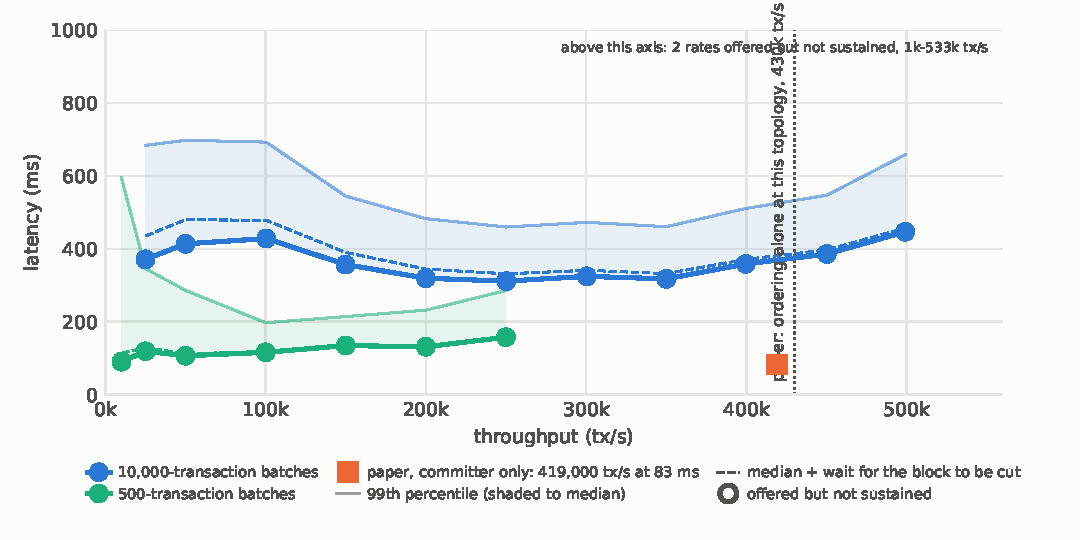
\includegraphics[width=\textwidth]{figures-e2e-batch/latency-throughput.pdf}
  \caption{Latency against throughput end to end, by batch size, on four shards with a volume per batcher. Marks as Fig.~\ref{fig:curve}.}
  \label{fig:e2ebatch}
\end{figure*}

\subsection*{Latency against throughput, by batch size}

Batch size is the latency--throughput knob here, and it trades one for the other almost exactly
(Fig.~\ref{fig:e2ebatch}), at the same workload again. Cutting the batch from \num{10000} transactions to 500 removes most of
the latency at every rate the two share --- p99 \SI{197}{\milli\second} against \SI{693}{\milli\second} at \num{100000} tps,
\SI{286}{\milli\second} against \SI{460}{\milli\second} at \num{250000}, and mean latency between a
quarter and a half of what large batches give. That is the predicted effect and its direction confirms the
mechanism: a batch a twentieth the size fills twenty times sooner, so the
\SI{500}{\milli\second} \texttt{BatchCreationTimeout} stops being what cuts it.

What it costs is the ceiling, and the reason is exact. The block rate tracks the offered rate
precisely --- 200 blocks a second at \num{100000} tps, 400 at \num{200000}, 500 at
\num{250000} --- and between 500 and 600 blocks a second the arm stops working. \num{250000} tps is
therefore not a transaction limit at all: it is $500 \times 500$, a \emph{block}-rate ceiling near
500 a second. At \num{10000} transactions a batch the same block rate would carry five million
transactions a second, which is why that configuration is limited by transactions instead and reaches
\num{499091}.

So the two configurations are bounded by different things, and the choice is a real trade rather than
a tuning win: small batches halve the latency and halve the ceiling.

\begin{figure*}[t]
  \centering
  
\includegraphics[width=\textwidth]{figures-e2e/size-throughput.pdf}
  \caption{Throughput against transaction size end to end, beside the published Figure 7b. Each point is annotated with the byte rate it implies.}
  \label{fig:size}
\end{figure*}

\subsection*{Throughput against transaction size}

Throughput falls with transaction size, but far more slowly than in the published sweep, and the byte
rate is what shows why (Fig.~\ref{fig:size}). The sweep keeps the same two read--write operations and
varies only the value each one carries, so the serialized envelope is \num{202} bytes plus twice that
value. The published measurement is bandwidth-bound past
\SI{300}{\byte}: each of its points sits within \SI{10}{\percent} of
\SI{120}{\mega\byte\per\second}, so its rate is simply bytes per second divided by size. This
deployment is not bandwidth-bound anywhere in the range. Its byte rate \emph{rises} with size, from
\SI{122}{\mega\byte\per\second} at \SI{300}{\byte} to \SI{410}{\mega\byte\per\second} at
\SI{4}{\kibi\byte}, because what it pays per transaction dominates what it pays per byte: halving the
transaction count at twice the size is a net gain. Throughput therefore falls about
\num{0.76}$\times$ per doubling rather than the \num{0.5}$\times$ a bandwidth-bound service gives.

The tabulated \SI{512}{\byte} figure is nominally above the \SI{300}{\byte} one, which is not a real
inversion: the \SI{300}{\byte} point's two holds span \numrange{408000}{443800} tps and
\SI{512}{\byte} sits inside that, so the sweep is flat between those sizes rather than rising. It is
the kind of difference the repeatability figure in Table~\ref{tab:size} exists to rule out.

Where that stops is measurable, and it is the assembler's disk. At \SI{4}{\kibi\byte} the arm delivers
\SIrange{113000}{123000}{} tps whether it is offered \num{118000} or \num{163200}, so throughput
plateaus near \num{120000} tps --- \SI{492}{\mega\byte\per\second} of envelope bytes --- with no
machine anywhere above \SI{54}{\percent} CPU, so it is not a processing limit. The highest rate that
also meets the latency bound, which is what Table~\ref{tab:size} reports, is lower still at
\num{100000} tps. The
assemblers at that point are writing \SIrange{527}{546}{\mega\byte\per\second} to their data
volume, against the \SI{529}{MiB/s} sequential write Table~\ref{tab:disk} measures on these
machines: the device is saturated. Each of the four assemblers writes the \emph{complete} block
stream, where a batcher writes only its own shard's share, so the assembler is where a byte rate
first meets a disk. At \SI{2}{\kibi\byte} the same figure is \SI{319}{\mega\byte\per\second},
three fifths of that ceiling, which is why that point holds cleanly and this one does not.

So the sweep has two regimes rather than one. Below \SI{2}{\kibi\byte} the arm is limited per
transaction and the byte rate climbs; at \SI{4}{\kibi\byte} it is limited per byte by one
component's disk, and the published bandwidth-bound model finally applies here too, at about four
times the bandwidth.

The consequence for the comparison is that only the direction is shared. Both lines fall, and this
one is above the published line at every size they have in common --- but it is a whole pipeline
against one of its parts, at four shards against two, so the gap is not a speedup and the shapes are
not measuring the same limit.

\begin{table}[t]
  \centering
  \footnotesize
  \caption{The size sweep end to end, with the evidence class of each point, since they do not all meet
  the same bar. A hold is tabulated in preference to a higher probe wherever both exist. At
  \SI{1}{\kibi\byte} and above a hold does not fit in one deployment: each assembler writes the
  complete block stream, so a \SI{485}{\giga\byte} volume fills in under twenty minutes at these byte
  rates, less than a rate search followed by a \SI{300}{\second} hold. The \SI{300}{\byte} point is
  the lower of two holds \SI{8.8}{\percent} apart, so all figures are given to three significant
  figures.}
  \label{tab:size}
  \begin{tabular}{@{}lrrl@{}}
    \toprule
    Size & Throughput (tx/s) & Byte rate & Evidence \\
    \midrule
    \SI{300}{\byte}  & \num{408000} & \SI{122}{MB/s} & two holds, lower one \\
    \SI{512}{\byte}  & \num{414000} & \SI{212}{MB/s} & confirmed hold \\
    \SI{1}{\kibi\byte} & \num{285000} & \SI{292}{MB/s} & probe; volume filled \\
    \SI{2}{\kibi\byte} & \num{156000} & \SI{319}{MB/s} & confirmed hold \\
    \SI{4}{\kibi\byte} & \num{100000} & \SI{410}{MB/s} & probe; disk-bound \\
    \bottomrule
  \end{tabular}
\end{table}

\section*{Storage characterisation}

Two properties of these volumes bound the results above, and both had to be measured: the volumes are
\texttt{virtio} devices reporting neither a model nor a meaningful rotational flag, so the backing
media cannot be identified from inside the guest. Table~\ref{tab:disk} gives \texttt{fio} 3.35 in the
four patterns this deployment produces.

First, ordering machines have half the disk bandwidth as well as half the cores, at almost exactly a
factor of two on every bandwidth row, at round figures repeating to four significant figures across
machines and volumes --- these are provisioned caps, not device characteristics, so a ceiling on that
arm must be read against the cap before it is attributed to ordering. The synchronous pattern is the exception, where the
ordering volumes are the faster of the two (\SI{297}{\micro\second} against \SI{395}{\micro\second}
at the median). Second, durability
is the expensive direction: making one \SI{4}{\kibi\byte} record durable with an \texttt{O\_DSYNC}
write costs about \SI{400}{\micro\second}, capping any per-record design near \num{2400} operations a
second, three orders of magnitude below the rates measured here. The ledger survives that only by
batching --- it appends a whole block and syncs every hundredth. Syncing alone is cheap by comparison,
an \texttt{fdatasync} after a buffered write returning in about \SI{0.08}{\milli\second}: it is the
write, not the barrier, that costs.

\begin{table}[t]
  \centering
  \footnotesize
  \caption{\texttt{fio} 3.35, \texttt{libaio}, \texttt{direct=1}, \SI{20}{\second} per pattern, run on
  a volume the deployment was not using at the time. Committer figures are the range across a database
  node and the sidecar. A synchronous engine caps fio's queue depth at 1 while still reporting the
  depth asked for, so the deep rows use \texttt{libaio}.}
  \label{tab:disk}
  \begin{tabular}{@{}llrr@{}}
    \toprule
    Pattern & Depth & Committer & Ordering \\
    \midrule
    \SI{1}{\mebi\byte} seq.\ write & 4  & \SI{1058}{MiB/s} & \SI{529}{MiB/s} \\
    \SI{4}{\kibi\byte} O\_DSYNC write & 1  & \num{2400} IOPS  & \num{3249} IOPS \\
    \SI{8}{\kibi\byte} rand.\ read & 32 & \num{126000} IOPS & \num{67689} IOPS \\
    \SI{8}{\kibi\byte} rand.\ write & 32 & \num{102000} IOPS & \num{51165} IOPS \\
    \bottomrule
  \end{tabular}
\end{table}

\section*{Threats to validity}

The load generator is the instrument, and in one figure it is the limit: its block preparation caps the
small-block curve in Fig.~\ref{fig:curve}. Elsewhere it is close to being one. At the end-to-end knee it runs at \SI{77}{\percent} of
its 64 cores against the busiest validator--committer's \SI{81}{\percent}, and on the
\SI{300}{\byte} size point at \SI{80}{\percent} against \SI{81}{\percent} --- tied, within the
noise. Every figure near \num{500000} tps should therefore be read as a bound on the pair, generator
and pipeline together, not on the pipeline alone. Separating them needs a second generator, and there
is no spare machine for one without taking it from the committer. A
knee is resolved to the search's \SI{8}{\percent} step, so it is a lower bound, drawn one-sided in
Fig.~\ref{fig:panels}. The baseline drifts \SI{10}{\percent} between days, so only same-day
comparisons are used, and within a day repeatability is no better: one configuration measured twice
gave holds \SI{8.8}{\percent} apart, and two configurations that are the same workload reached by
separate searches differed by \SI{7.9}{\percent}. A difference under about a tenth is therefore not a
result here, and no claim in this section rests on one.

A ladder climbs on a single deployment, so rate and table fill rise together along it. Repeating the
rates around the knee on fresh deployments moves the boundary by less than the spread above, so the
knee is a property of the rate; the tail near it does grow with fill. Every rung records the fill it
ran against.

\end{document}
